\section{符合矩阵与能级建立}\label{sec:5-6}

在在束 $\gamma$ 谱学与核衰变测量中，单探测器的单谱仅能提供反应产生的各特征光子的一维发射能量与总产额。然而，核反应通常布居了复杂的能级网络，数十条甚至上百条 $\gamma$ 跃迁同时发生，造成一维能谱严重重叠。为了从错综复杂的谱线中重构出原子核的量子能级序列并建立自洽的衰变纲图，核心的实验手段是利用多探测器阵列记录的\emph{$\gamma\text{-}\gamma$ 符合关系}。

第~5.4~节讨论了基于 CFD 过零插值的高精度时间戳提取，第~5.5~节阐明了硬件触发、FIFO 缓存与联合活时间的因果界限。当数据流记录至存储介质后，离线物理分析的第一步便是通过时间对准构建物理符合事件，并将多重事件填充为二维或高维符合矩阵。若对矩阵填充测度、偶然符合扣除、非对称门选背景以及级联拓扑逻辑缺乏充分把握，容易引入两类代表性的系统假象：其一，将同一多重事件对称填充产生的统计相关性误当成各独立格点的独立泊松起伏；其二，混淆符合关联与级联因果次序，将旁路跃迁或能量重叠双重峰（Doublet）误判为直接级联。本节从离线事件重构与符合时间窗出发，推导二维对称与非对称矩阵的填充测度，建立瞬发--偶然符合扣除与误差协方差传播公式，剖析能谱门选背景扣除与假符合排除方法，并阐明建立原子核能级纲图的拓扑闭合准则。

\subsection{事件构建、时间对准与符合窗口}\label{subsec:5-6-1}

在数字化数据获取中，各探测通道由独立的 ADC 和 FPGA 独立运行并输出带有局域时间戳的列表模式数据字（见第~5.5~节）。离线分析的首要任务是进行事件构建（Event Building）：
\begin{enumerate}
\item 时间对准与通道延迟校正：
各探测通道由于电缆长度、探测器前放上升时间以及晶体几何位置的微小差异，对同一物理瞬发事件记录的时间戳存在固定纳秒级的相对走动。必须通过已知放射源（如 $^{60}\mathrm{Co}$ 的 $1173\text{--}1332\,\text{keV}$ 级联）离线测量各通道间的时间差谱 $\Delta t_{ij} = t_i - t_j$，提取各通道的时间偏置校正量 $\delta t_i$，使时间对准后的瞬发符合峰中心精确归零。
\item 符合时间窗口 $\Delta T_{\mathrm{coin}}$ 的选取权衡：
将时间排序后的数据流按时间间隔划分物理事件。若相邻击中时间满足 $|(t_i - \delta t_i) - (t_j - \delta t_j)| \le \Delta T_{\mathrm{coin}}$，则判决属于同一个物理退激事件。
\begin{itemize}
\item 窗口宽度的下限受到探测系统本征时间分辨率（第~5.4~节的 FWHM 展宽）的物理制约，过窄的窗口会截断瞬发符合峰的两翼，导致特定能量或角度的有效符合计数发生不对称损失；
\item 窗口宽度的上限受到在束偶然符合计数率的直接压制：偶然符合计数正比于窗口宽度 $\Delta T_{\mathrm{coin}}$，过宽的窗口会导致大量不相干的背景反应事件混入真符合网络，显著恶化谱线信噪比。在典型的在束大阵列实验中，瞬发符合窗口通常优化设定为 $30\text{--}100\,\text{ns}$。
\end{itemize}
\end{enumerate}
离线事件构建是在计算机中对已记录数据流进行的关联重构。前端未保存的事件信息，不能仅靠离线重组恢复；对于已经保存的数据，时间窗的选取则需要权衡真符合效率与偶然本底污染。

\subsection{二维对称与非对称符合矩阵的填充测度}\label{subsec:5-6-2}

当一个物理事件在符合时间窗口 $\Delta T_{\mathrm{coin}}$ 内包含 $M_\gamma = n$ 个被鉴别的特征光子，其观测能量集合为 $\{E_1, E_2, \dots, E_n\}$。离线分析通常将这些事件填充到二维矩阵 $M(E_x, E_y)$ 中。
\begin{enumerate}
\item 二维对称符合矩阵（Symmetric $\gamma\text{-}\gamma$ Matrix）：
用于分析核能级纲图的共性级联关系与相对跃迁强度。为了保证 $x$ 轴与 $y$ 轴对于探测器身份的等价性，对于包含多重度 $M_\gamma = n$ 的单次物理事件，其无序数对共有 $n(n - 1)/2$ 对。在构建对称矩阵时，对每一对指标 $i < j$，分别在坐标点 $(E_i, E_j)$ 与转置镜像点 $(E_j, E_i)$ 处各填入计数 1，使总填入条目数恰为：
\begin{equation}\label{eq:5-6-ordered-pairs}
N_{\mathrm{entries}} = 2 \times \frac{n(n - 1)}{2} = n (n - 1).
\end{equation}
在此规则下，矩阵满足转置对称性 $M(E_x, E_y) = M(E_y, E_x)$。
特别地，当且仅当一个物理事件中包含两个能量相同的独立跃迁光子时（如核退激级联中恰好发射了两颗能量简并的 $\gamma$ 光子并在不同探测单元中记录），该事件才对等填入主对角线格元 $(E_i, E_i)$ 上（须注意排除由于相邻晶体间康普顿散射串扰或假相加引起的非独立光子伪计数）。
\item 二维非对称符合矩阵（Asymmetric Coincidence Matrix）：
用于提取特定几何角度的物理各向异性或偏振信息。例如在方向角关联（DCO）或定向角分布（ADO）测量中（肖骁 2019 硕士学位论文，PDF 第~23--24~页，印刷第~15--16~页~\cite{xiao-xiao-2019-high-spin-74as-thesis}）：
\begin{itemize}
\item 矩阵 $x$ 轴限定为全部探测器测得的光子能量，而 $y$ 轴限定为特定角度（如 $90^\circ$ 或 $135^\circ$）探测器记录的光子能量；
\item 或者将 $x$ 轴与 $y$ 轴分别绑定为小角度（如 $30^\circ/150^\circ$）与近 $90^\circ$ 探测器组。
\end{itemize}
在此情形下，矩阵不具备对称性，$M(E_x, E_y) \neq M(E_y, E_x)$，单次多重事件填充时仅将符合角几何条件的光子对按物理通道定向填入。
\end{enumerate}

\subsection{瞬发--偶然符合扣除与误差协方差传播}\label{subsec:5-6-3}

在束实验中，符合时间窗口内捕获的光子对不仅包含源自同一次核退激的真符合事件，还叠加了两次不相干核反应发射的光子偶然落入同一时间窗的偶然符合（Random Coincidence）事件。

在相对时间差谱 $\Delta t$ 上，分别设置瞬发时间窗（Prompt Window，宽度为 $\Delta T_P$）与位于瞬发峰外侧较远处平坦区域的偶然时间窗（Random Window，宽度为 $\Delta T_R$）。分别填充生成二维瞬发矩阵 $P(E_x, E_y)$ 与二维偶然矩阵 $R(E_x, E_y)$。
净真符合矩阵的统计估计量定义为：
\begin{equation}\label{eq:5-6-prompt-random}
S(E_x, E_y) = P(E_x, E_y) - a R(E_x, E_y),
\end{equation}
其中时间归一化比例因子为：
\begin{equation}\label{eq:5-6-norm-factor}
a \equiv \frac{\Delta T_P}{\Delta T_R}.
\end{equation}

在误差传播与统计推断中，应考虑以下统计原则：
\begin{enumerate}
\item 误差传递与 Delta 方法展开：
若归一化因子 $a = \Delta T_P / \Delta T_R$ 由预设的时间门宽比例确知为固定常数，则有限偶然计数 $R$ 本身并不引起 $a$ 的统计不确定度。下面的方差公式由本稿按所列统计假设推导。若瞬发与偶然时间差门中的计数可近似视为相互独立的泊松变量，理论总体方差满足：
\begin{equation}\label{eq:5-6-var-population}
\mathrm{Var}(S) = \mu_P + a^2 \mu_R,
\end{equation}
其中 $\mu_P, \mu_R$ 为瞬发与偶然计数的真实泊松期望均值。在实验数据处理中，可用代入估计量（Plug-in Estimator）评估方差：
\begin{equation}\label{eq:5-6-var-net}
\widehat{\mathrm{Var}}(S) = P + a^2 R.
\end{equation}
若归一化因子 $a$ 依赖于从实测时间谱或无相干本底能谱中拟合得到的参数，其方差 $\mathrm{Var}(a)$ 与相关协方差进入误差链。在更一般的非线性参数设定下，由一阶 Delta 方法导出的全协方差传递式为：
\begin{equation}\label{eq:5-6-var-cov-expanded}
\begin{aligned}
\mathrm{Var}(S)\simeq{}&\mathrm{Var}(P)+a^2\mathrm{Var}(R)+R^2\mathrm{Var}(a)\\
&-2a\mathrm{Cov}(P,R)-2R\mathrm{Cov}(P,a)+2aR\mathrm{Cov}(R,a).
\end{aligned}
\end{equation}
需要注意：式~\eqref{eq:5-6-var-net} 是方差的样本估计量，并非总体方差的绝对恒等式；包含多重事件或加权对称填充的矩阵格点计数并不自动服从独立泊松点过程。
\item 负计数的统计属性认知：
在弱谱线区域，本底扣除后的估计量 $S = P - aR$ 出现负值属于正常的统计下涨落。需要明确：仅在假定本底扣除比例 $a$ 准确且无通道泄漏的条件下，$S$ 在纯本底无信号的零假设（Null Hypothesis）下期望才为零；若 $a$ 源于拟合估计并包含相关性，其实际估计值可能存在残余偏置。在弱谱线能区出现负估计值不应将其视为物理负强度，亦不应在解谱前将负值强制置零（强制截断会导致正向系统偏置）。
\end{enumerate}

\subsection{能谱门选、背景扣除与假符合排除}\label{subsec:5-6-4}

建立了二维符合矩阵后，研究人员通过在一维轴上对特定能量的谱峰设置门窗（Gate），截取并投影出与其存在符合级联关系的退激能谱。

设对能级上方或下方的跃迁 $\gamma_1$（峰位为 $e_0$）设置总峰门（Gross Peak Gate），门宽区间为 $[e_0 - \delta_1, e_0 + \delta_1]$，宽度为 $w_p = 2\delta_1$。投影到另一能量轴上得到的总门谱 $G(E_y)$ 包含了两个物理成分：
$$
\begin{aligned}
G(E_y)={}&\text{与全能峰 }e_0\text{ 级联的真符合谱}\\
&+\text{与 }e_0\text{ 峰下连续康普顿本底符合的伪符合谱}.
\end{aligned}
$$
为了估计峰门内的连续本底，在峰位两侧无特征峰的区域分别设置左背景门与右背景门。设左背景门中心为 $e_L$、宽度为 $w_L$、投影谱为 $B_L(E_y)$，右背景门中心为 $e_R$、宽度为 $w_R$、投影谱为 $B_R(E_y)$。左右背景门单位能量的计数密度分别为 $B_L(E_y)/w_L$ 与 $B_R(E_y)/w_R$（量纲为计数$/\mathrm{keV}$）。以下为本稿的局域线性插值推导：假定对固定的 $E_y$，本底密度在这几个能量窗覆盖范围内近似为能量的一次函数，各窗以所列中心对称积分。于是，窗内平均密度等于中心密度，将两侧密度内插至峰位中心 $e_0$，再乘以峰门宽度 $w_p$，得到：
\begin{equation}\label{eq:5-6-gate-sub}
S_{\mathrm{gated}}(E_y) = G(E_y) - w_p \left[ \lambda_L \frac{B_L(E_y)}{w_L} + \lambda_R \frac{B_R(E_y)}{w_R} \right],
\end{equation}
其中无量纲内插权重系数满足：
\begin{equation}\label{eq:5-6-gate-weights}
\lambda_L = \frac{e_R - e_0}{e_R - e_L}, \quad \lambda_R = \frac{e_0 - e_L}{e_R - e_L} = 1 - \lambda_L.
\end{equation}
式~\eqref{eq:5-6-gate-sub} 中括号内各项为单位能量道宽的本底计数密度，乘以宽度 $w_p$ 后量纲与门谱计数一致。当双侧背景窗宽度相等（$w_L = w_R = w_b$）且对称放置（$e_0 - e_L = e_R - e_0 \implies \lambda_L = \lambda_R = 1/2$）时，式~\eqref{eq:5-6-gate-sub} 退化为常见的等权平均形式 $S_{\mathrm{gated}} = G - \frac{w_p}{2 w_b}(B_L + B_R)$。若背景门宽度不等，则不能直接平均原始计数 $B_L, B_R$，而必须通过计数密度归一。

在执行门谱分析时，应注意以下导致假符合（False Coincidence）的复杂情形：
\begin{enumerate}
\item 本底形状的非线性结构：
第~5.2~节阐明了康普顿边缘与散射峰的微观机理。在实际锗谱中，全能峰下方的本底未必接近一次函数；若背景门跨越了邻近强跃迁的康普顿边缘或后向散射峰，式~\eqref{eq:5-6-gate-sub} 的线性假设便可能失效，净门谱会出现残余峰或下凹。吴治华教材第10章第六节之四（印刷第292--294页，PDF第300--302页）及图10.38给出了符合矩阵、开门投影和级联比较的实验分析框架~\cite{book-wu-nuclear-experiment-methods}；这里的双侧密度插值公式及其统计误差展开是本稿在该框架下的条件推导。
\item 重叠双重峰（Doublet）的解谱污染：
当两个能量相近的跃迁存在于不同谱带中形成重叠双重峰时，对其中一个峰设门必然同时接收另一个峰的符合通道。此时必须借助不同侧带的高位或低位纯净单门进行交叉解叠。
\item 平行分支与反符合排除（Anti-Coincidence Verification）：
符合关系的逻辑证伪同样重要。Wakudyanaye 论文（硕士论文，PDF 第~62--63~页，印刷第~51--52~页~\cite{wakudyanaye-2022-triaxiality-rotational-bands-133ce}）给出了旁路分支的判定逻辑：当对 $871\,\text{keV}$ 设门时未观察到 $490\,\text{keV}$ 与 $380\,\text{keV}$ 跃迁，但对 $936\,\text{keV}$ 设门时这两条跃迁清晰可见，作者由此判定 $490\,\text{keV}$ 与 $380\,\text{keV}$ 跃迁处于与 $871\,\text{keV}$ 平行的退激支路上。必须明确：在有限计数的门谱中未观察到某峰，受探测效率、分支比上限、本底涨落及能门重叠等实验检测灵敏度的约束，不能在缺乏灵敏度与计数上限评估的前提下直接断言为绝对反符合；在实验谱学中，它提供的是支持特定分支拓扑的条件性证据，而非脱离灵敏度边界的确定性排除。
\end{enumerate}

图~\ref{fig:5-6-coincidence-topology} 给出了一个规范的教学模型，直观展示了交叉跃迁（Crossover）、平行旁路分支以及双重峰在符合矩阵门谱分析中的判据逻辑。

\begin{figure}[!htbp]
\centering
%
  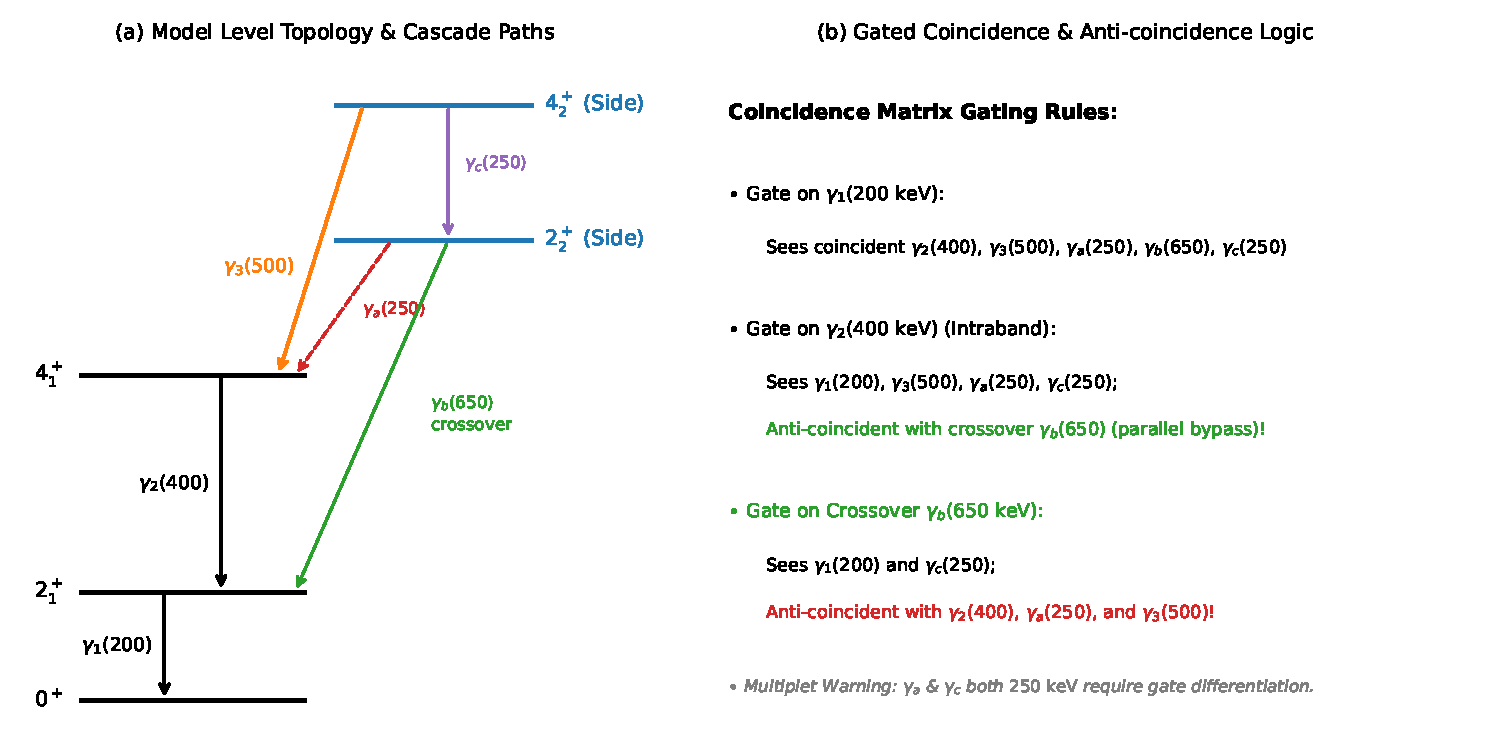
\includegraphics[width=0.92\textwidth]{Img/coincidence-level-scheme-model.pdf}%
\caption[典型核能级符合拓扑与门选反符合判据模型]{典型核能级符合拓扑与门选反符合判据模型（教学模型，基于参数化合成逻辑生成，各跃迁能量差、自旋多极选择定则及级联路径均经程序自洽验证）。(a) 展示包含基态带（$0^+ \to 2_1^+ \to 4_1^+$）与准 $\gamma$ 侧带（$2_2^+, 4_2^+$）的能级拓扑结构，包含带内与带间跃迁 $\gamma_1(200, E2), \gamma_2(400, E2), \gamma_3(500, M1+E2)$、侧向跃迁 $\gamma_a(250, E2), \gamma_c(250, E2)$ 以及交叉跃迁 $\gamma_b(650, M1+E2)$；(b) 给出符合门选逻辑：对 $\gamma_1$ 设门可见全部相连级联；对 $\gamma_2$ 设门可见 $\gamma_1, \gamma_3, \gamma_a, \gamma_c$，在理想衰变网络模型中与交叉跃迁 $\gamma_b$ 呈现拓扑反符合（平行旁路，无公共级联路径）；对交叉跃迁 $\gamma_b$ 设门可见 $\gamma_1, \gamma_c$，在理想模型中与 $\gamma_2, \gamma_a, \gamma_3$ 呈现拓扑反符合（在实验谱分析中，未观测到谱峰受探测限与统计涨落约束，与理想图模型的拓扑反符合性质有明确区分）；同时标示了 $\gamma_a$ 与 $\gamma_c$ 同为 $250\text{ keV}$ 时的双重峰（Doublet）门选消歧判据。注意此处为规范教学模型，非特定未知实验测量拟合）。}
\label{fig:5-6-coincidence-topology}
\end{figure}

\subsection{符合拓扑、级联排序与能级纲图建立原则}\label{subsec:5-6-5}

在谱学反演中必须牢记核心逻辑边界：\emph{两个特征 $\gamma$ 射线在谱图中存在符合关联，仅能证明二者同处于一个级联退激网络之中，并不自动确定二者的相对次序，更不代表二者是直接相连的相邻跃迁}。在排除反应伴生碎片、偶然相加与探测器散射串扰等假符合污染后，符合关系确认的是退激网络的拓扑连通性。从符合计数上升为可信能级纲图，必须同时满足以下拓扑闭合准则：
\begin{enumerate}
\item 能量守恒与 Ritz 组合原理（Ritz Combination Principle）：
在同一核素衰变网络中，两能级之间的能量差在计入微小的核反冲修正与实验刻度误差后，经由多步级联退激的跃迁能量代数和必须与交叉单跃迁（Crossover Transition）在测量不确定度内精确吻合。设各级联步跃迁能量为 $E_k$，反冲修正后的能级能量差为 $\Delta E_k = E_k + \frac{E_k^2}{2 M c^2}$，交叉跃迁对应能级差 $\Delta E_{\mathrm{crossover}} = E_{\mathrm{crossover}} + \frac{E_{\mathrm{crossover}}^2}{2 M c^2}$，则能量守恒要求 $\Delta E_{\mathrm{crossover}} = \sum_{k=1}^m \Delta E_k$。在观测光子能量尺度上，这表达为：
\begin{equation}\label{eq:5-6-ritz-combination}
E_{\mathrm{crossover}} = \sum_{k=1}^m E_k - \Delta E_{\mathrm{recoil}},
\end{equation}
其中 $\Delta E_{\mathrm{recoil}} \equiv \frac{E_{\mathrm{crossover}}^2}{2 M c^2} - \sum_{k=1}^m \frac{E_k^2}{2 M c^2} > 0$ 为交叉跃迁与多步级联反冲动能损失总和的差值（对于质量数 $A \approx 130$ 的核素，$1\,\text{MeV}$ 跃迁的反冲能量约为 $4\,\text{eV}$，在常规高分辨率高纯锗能谱中通常小于测量误差，但多步高能级联累积时仍应注意其物理定义）。
\item 强度平衡与开闭流分析：
在稳态衰变平衡与连续束流照射下，对中间能级 $|i\rangle$，其净布居速率由直接反应布居、侧向未观测馈入、离散级联注入与全部退激分支共同维持平衡：
\begin{equation}\label{eq:5-6-intensity-balance}
I_{\mathrm{direct}}(i) + I_{\mathrm{side}}(i) + \sum_{k} I_{\mathrm{tot}, k}^{\mathrm{in}} = \sum_{j} I_{\mathrm{tot}, j}^{\mathrm{out}} + I_{\mathrm{loss}}(i).
\end{equation}
仅在无直接输入且无未观测漏支的理想闭合子体系中，才近似有 $\sum I_{\mathrm{in}} \approx \sum I_{\mathrm{out}}$。总跃迁强度 $I_{\mathrm{tot}}$ 必须计入内转换系数 $\alpha_{\mathrm{IC}}$：
\begin{equation}\label{eq:5-6-itot-expansion}
I_{\mathrm{tot}, k} = I_{\gamma, k} (1 + \alpha_{\mathrm{IC}, k}).
\end{equation}
若某能级观测到的光子流入明显小于流出，常暗示存在来自高能连续区或侧带的未分辨馈入；若流入显著大于流出，则指示存在强内转换的未观测低能跃迁（$\alpha_{\mathrm{IC}} \gg 1$）。需要特别说明：在真正达到稳态且完全时间积分的闭合衰变网络中，总强度是严格守恒的，寿命本身并不会在稳态下消灭流量；若核态存在长寿命异能态延迟（$\tau_{\mathrm{isomer}} > \Delta T_{\mathrm{coin}}$）或处于脉冲束流的非稳态建立期，下游跃迁强度在有限时间门宽内将呈现表观的流入/流出不平衡，数据分析时须明确时间积分窗口与稳态建立的边界条件（肖骁 2019 硕士学位论文，PDF 第~24--26~页，印刷第~16--18~页~\cite{xiao-xiao-2019-high-spin-74as-thesis}）。
\item 级联次序的时间与强度反演：
单靠两个相互符合的光子能量无法确定相对上下次序。确定级联跃迁的上下次序依赖于强度单调递减规律（在无严重侧向注入的前提下，沿转动带自上而下退激时跃迁总强度单调累增）、从不同侧带分支汇入点的几何连接特征，以及第~5.4~节讨论的纳秒/皮秒时间差符合测量（若两态寿命差异足以在符合时间谱上分辨因果先后）。
\item 自旋宇称指定的独立证据输入：
能级纲图中每个激发态的自旋与宇称 $I^\pi$ 不能仅凭符合谱能量直接指认。能量符合建立的是能级拓扑连通图；能级自旋宇称的最终锁定，通常综合输入第~5.7~节的在束角分布 $W(\theta)$ / DCO（确定多极阶数 $L$ 与混合比 $\delta$）、Compton 偏振不对称度 / 内转换系数（确定电磁宇称性质 $\pi$），并结合已知的基态或基准能级锚定与选择定则。必须指出：自旋宇称指定的判定并不普遍要求测得能级绝对寿命 $\tau$。能级寿命 $\tau$ 与绝对折合跃迁几率 $B(XL)$ 是测定核结构波函数微观跃迁强度的关键物理量（见第~5.8~节），但由角分布与偏振给出的多极性与自旋指认属于辐射角动量与空间对称性约束，二者在实验证据链中具有明确的层次分工。
\end{enumerate}
通过符合拓扑、能量封闭、强度守恒与角分布偏振的多维交叉印证，才能将实验离线数据最终固化为经得起检验的确定核结构能级纲图。
